\documentclass{article}

\usepackage{graphicx}
\usepackage{tikz}
\usepackage{tikzsymbols}
\usetikzlibrary{calc,patterns,shapes.geometric}
\pagestyle{empty}
\usepackage[margin=0pt]{geometry}
\geometry{papersize={14in,12in}}

\def\centerarc[#1](#2)(#3:#4:#5){\draw[#1] ($(#2)+({#5*cos(#3)},{#5*sin(#3)})$) arc (#3:#4:#5);}

\begin{document}
	\begin{figure}
		\centering
		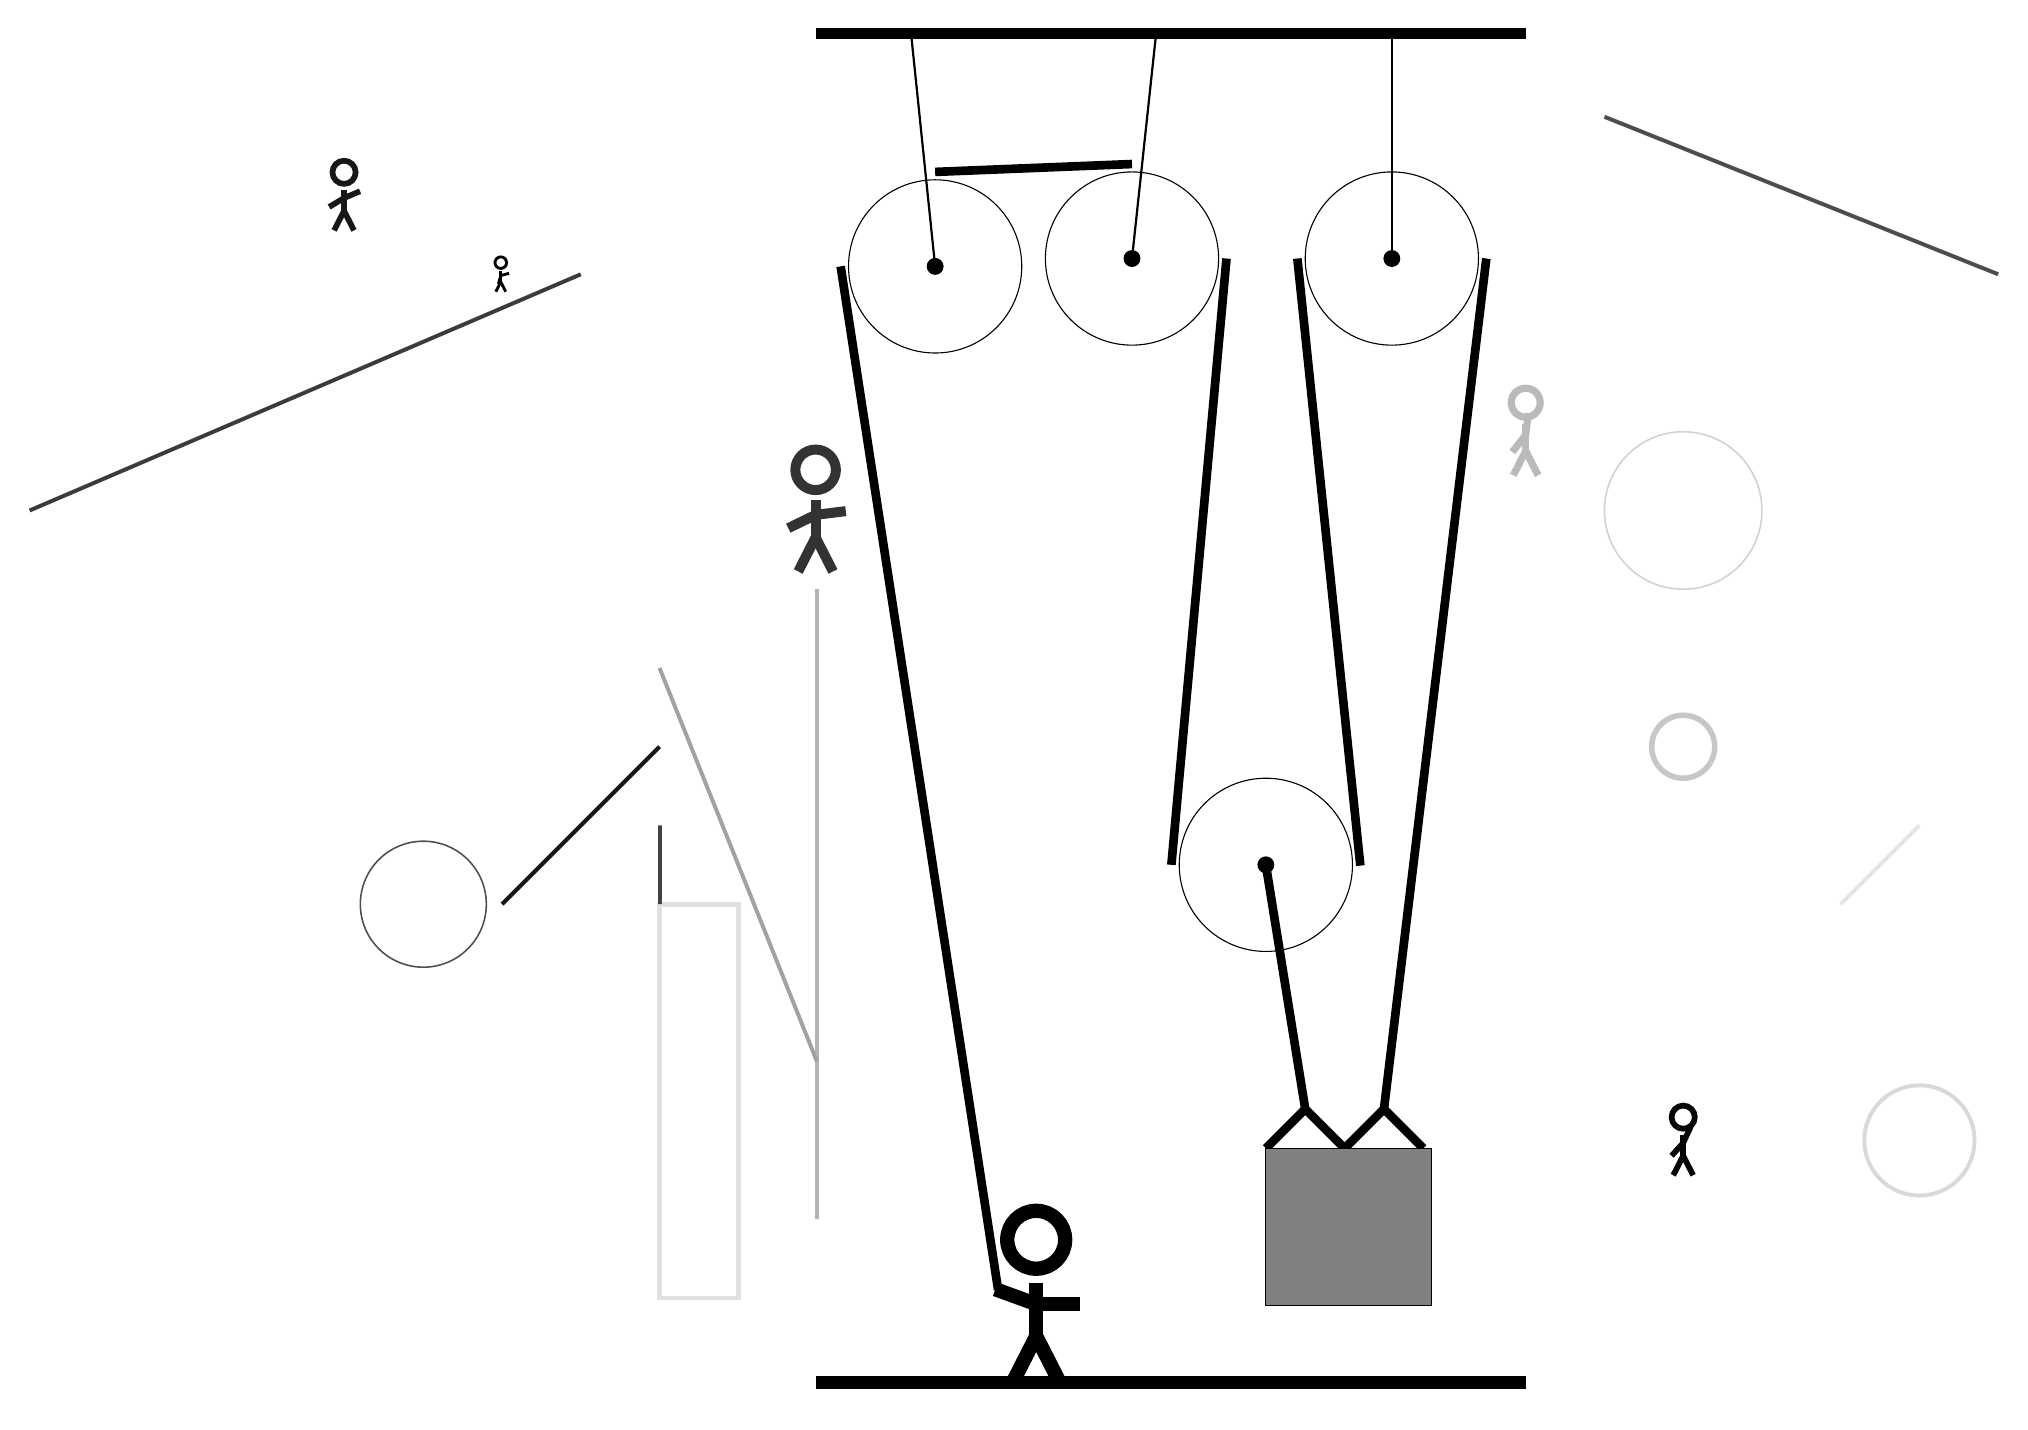
\begin{tikzpicture}
			%%%%% START %%%%%
			
			\draw[fill=black] (-3, 14) rectangle (6, 14.125);
			
			\draw [line width=0.2mm, color=black!69](-8, 3) circle (0.8);
			
			\node[line width=0.3mm, color=black!100] at (-7, 11) {\Strichmaxerl[2][74][15]};
			\draw[line width=0.5mm, color=black!29] (-3, -1) rectangle (-3, 7);
			\draw[line width=0.6mm, color=black!12] (-4, 3) rectangle (-5, -2);
			\draw[line width=0.5mm, color=black!74] (-5, 4) rectangle (-5, 3);
			
			\node[line width=0.5mm, color=black!27] at (6, 9) {\Strichmaxerl[5][52][83]};
			\draw[line width=0.5mm, color=black!70](7, 13) -- (12, 11);
			\node[line width=0.2mm, color=black!80] at (-3, 8) {\Strichmaxerl[7][26][7]};
			\draw[line width=0.5mm, color=black!37](-5, 6) -- (-3, 1);
			\draw[line width=0.5mm, color=black!91](-5, 5) -- (-7, 3);
			
			\draw[line width=0.5mm, color=black!77](-6, 11) -- (-13, 8);
			\draw [line width=0.7mm, color=black!22](8, 5) circle (0.4);
			\draw [line width=0.2mm, color=black!18](8, 8) circle (1.0);
			
			\draw[line width=0.5mm, color=black!10](11, 4) -- (10, 3);
			\draw [line width=0.5mm, color=black!15](11, 0) circle (0.7);
			\node[line width=0.3mm, color=black!91] at (-9, 12) {\Strichmaxerl[4][31][23]};
			\node[line width=0.3mm, color=black!98] at (8, 0) {\Strichmaxerl[4][48][65]};
			
			\draw (1, 11.2) circle (1.1);
			\draw[fill=black] (1, 11.2) circle (0.1);
			\draw[thick] (1, 11.2) -- (1.3, 14);
			
			\draw (4.3, 11.2) circle (1.1);
			\draw[fill=black] (4.3, 11.2) circle (0.1);
			\draw[thick] (4.3, 11.2) -- (4.3, 14);
			
			\draw (2.7, 3.5) circle (1.1);
			\draw[fill=black] (2.7, 3.5) circle (0.1);
			
			\draw[line width=1.1mm]  (2.7, -0.1) -- (3.2, 0.4) -- (3.7, -0.1) -- (4.2, 0.4) -- (4.7, -0.1);
			\draw[fill=black!50] (2.7, -0.1) rectangle (4.8, -2.1);
			
			\draw (-1.5, 11.1) circle (1.1);
			\draw[fill=black] (-1.5, 11.1) circle (0.1);
			\draw[thick] (-1.5, 11.1) -- (-1.8, 14);
			
			\draw[line width=1.1mm](-0.7, -1.9) --  (-2.7, 11.1);
			\centerarc[line width=1.1mm](-1.5, 11.1)(90:180:1.2000000000000002);
			\draw[line width=1.1mm](-1.5, 12.3) -- (1, 12.4);
			\centerarc[line width=1.1mm](1, 11.2)(0:90:1.2000000000000002);
			\draw[line width=1.1mm](2.2, 11.2) -- (1.5, 3.5);
			\centerarc[line width=1.1mm](2.7, 3.5)(180:370:1.2000000000000002);
			\draw[line width=1.1mm] (3.9, 3.49) -- (3.1, 11.2);
			\centerarc[line width=1.1mm](4.3, 11.2)(0:180:1.2000000000000002);
			\draw[line width=1.1mm](4.2, 0.4) -- (5.5, 11.2);
			\draw[line width=1.1mm] (3.2, 0.4) -- (2.7, 3.5);
			
			\node at (-0.2, -2) {\Strichmaxerl[10][-20][0]};
			
			\draw[fill=black] (-3, -3) rectangle (6, -3.15);
			
			%%%%% END %%%%%
		\end{tikzpicture}
	\end{figure}	
\end{document}